% VLDB WORKSHOP template version of 2024-05-15 enhances the ACM template, version 1.7.0:
% https://www.acm.org/publications/proceedings-template

\documentclass[sigconf, nonacm]{acmart}
\usepackage{xspace}
\usepackage{algorithm}
\usepackage{algorithmic}
\makeatletter
\@ACM@balancefalse
\makeatother

\newcommand\vldbyear{2026}
\newcommand\vldbworkshop{ADS 2026: The Joint Workshop on Agentic Data Systems and Data-Centric AI (The 1st ADS \& 3rd DATAI)}
\newcommand\vldbauthors{\authors}
\newcommand\vldbtitle{\shorttitle}
\newcommand\vldbavailabilityurl{}
\newcommand\vldbpagestyle{plain}

\newcommand{\sys}{\textsc{DDPAgent}\xspace}
\newcommand{\noop}{\textsc{No-op}\xspace}
\newcommand{\repair}{\textsc{Repair}\xspace}
\newcommand{\deleteop}{\textsc{Delete}\xspace}
\newcommand{\replaceop}{\textsc{Replace}\xspace}
\newcommand{\fullops}{\textsc{FullOps}\xspace}
\newcommand{\syssel}{\textsc{DDPAgent-Sel}\xspace}
\definecolor{rankFirst}{RGB}{184,49,47}
\definecolor{rankSecond}{RGB}{32,100,171}
\definecolor{algcomment}{rgb}{0,0.25,0}
\newcommand{\best}[1]{\textcolor{rankFirst}{\textbf{#1}}}
\newcommand{\runner}[1]{\textcolor{rankSecond}{\textbf{#1}}}
\newcommand{\algstage}[1]{\textcolor{algcomment}{\textit{#1}}}
\newtheorem{definition}{Definition}

\begin{document}

\title{\sys for Demand-Driven Data Preparation via Agentic Action Allocation and Operator-Grounded Execution}

\author{Zekai Qian}
\affiliation{%
  \institution{Harbin Institute of Technology, China}
}
\email{qzk010728@gmail.com}

\author{Xiaoou Ding}
\authornote{Corresponding author.}
\affiliation{%
  \institution{Harbin Institute of Technology, China}
}
\email{dingxiaoou@hit.edu.cn}

\author{Hongzhi Wang}
\affiliation{%
  \institution{Harbin Institute of Technology, China}
}
\email{wangzh@hit.edu.cn}

\begin{abstract}
Agentic data systems can invoke many data-cleaning operators, but they still lack a task-level mechanism for deciding which intervention a downstream task needs. In machine-learning pipelines, repairing a cell, deleting a record, replacing a value, applying all operators, or preserving the dirty input may lead to different utility under different metrics, data states, and costs.
We present \sys, a demand-driven data preparation framework that separates action-family allocation from operator-grounded execution. Given a task demand, \sys trains a hierarchical allocator without additional human labels for action selection, assigns high-level cleaning actions such as \noop, \repair, \deleteop, and \replaceop to candidate units, and compiles the selected actions into executable operator workflows with provenance. Downstream validation then chooses among conservative rollback to \noop, selective action execution, and intensive \fullops execution.
The paper makes four contributions. It introduces a task-demand formulation that treats preservation and full execution as valid agent decisions, connects zero-new-label action allocation with action-indexed operator networks, records action, workflow, operator, and operation provenance, and evaluates the design on five native-error datasets plus 40 mixed-error injected settings. The injected task tables have average cell-level error rate 1.58\%, average record-level error rate 17.78\%, and maximum record-level error rate 50.90\%. Against named fixed cleaning methods, \sys has the highest average utility and is ranked first or second on almost every native and injected aggregate row. The results show that data preparation is not monotone in cleaning strength. Some tasks demand selective repair, some demand broad operator execution, and some are best served by preserving the data after validation.
\end{abstract}

\maketitle

%%% do not modify the following VLDB block %%
%%% VLDB block start %%%
\pagestyle{\vldbpagestyle}
\begingroup\small\noindent\raggedright\textbf{VLDB Workshop Reference Format:}\\
\vldbauthors. \vldbtitle. VLDB \vldbyear\ Workshop: \vldbworkshop.\\
\endgroup
\begingroup
\renewcommand\thefootnote{}\footnote{\noindent
This work is licensed under the Creative Commons BY-NC-ND 4.0 International License. Visit \url{https://creativecommons.org/licenses/by-nc-nd/4.0/} to view a copy of this license. For any use beyond those covered by this license, obtain permission by emailing \href{mailto:info@vldb.org}{info@vldb.org}. Copyright is held by the owner/author(s). Publication rights licensed to the VLDB Endowment. \\
\raggedright Proceedings of the VLDB Endowment. \\
}\addtocounter{footnote}{-1}\endgroup
%%% VLDB block end %%%

%%% do not modify the following VLDB block %%
%%% VLDB block start %%%
\ifdefempty{\vldbavailabilityurl}{}{
\vspace{.3cm}
\begingroup\small\noindent\raggedright\textbf{VLDB Workshop Artifact Availability:}\\
The source code, data, and/or other artifacts have been made available at \url{\vldbavailabilityurl}.
\endgroup
}
%%% VLDB block end %%%

\section{Introduction}

Data-centric AI has made data quality a first-order design problem rather than a preprocessing detail~\cite{jarrahi2023datacentric,jakubik2024datacentric}. Dirty, missing, inconsistent, or biased records can dominate downstream model behavior even when the model architecture is unchanged~\cite{abedjan2016detecting,krishnan2016activeclean,krishnan2017boostclean}. Existing data cleaning research has developed many ways to detect and repair erroneous cells, including probabilistic inference, contextual repair, rule reasoning, and mixed-error workflow coordination~\cite{rekatsinas2017holoclean,mahdavi2019raha,mahdavi2019baran,ni2024automatic}. These methods provide concrete operators for data-centric systems, but they do not by themselves determine which intervention a downstream task needs.

The missing layer is a task-level controller that decides whether the current task demands repair, deletion, replacement, preservation, or full operator execution before an operator workflow is compiled. This decision is not monotone in the amount of cleaning. Repairing every suspicious cell may increase cell-level correctness but can erase rare patterns or overfit to an imperfect reference. Deleting all suspicious rows may remove harmful records but can collapse sample diversity. Automatic replacement is cheap and scalable, yet it can propagate systematic errors when the value estimator is misaligned with the target metric. Conversely, leaving data unchanged is not always a weak baseline. In a governed workflow, it is a rollback decision when validation finds limited data-side gain. Full operator execution is the opposite regime, indicating that broad preparation has higher validation utility than selective pruning.

Consider a user who wants to train a downstream classifier over a dirty tabular dataset containing typographical errors, missing values, outliers, and dependency violations. A conventional cleaning pipeline asks which cleaner should be run and in what order. A task-driven user asks which records or cells are worth changing for the downstream model. A typo in a high-impact feature may need repair. A suspicious row with implausible values may need deletion. A missing value in a low-sensitivity feature may be safely replaced by an automatic estimator. A rare but valid boundary example should be preserved even if a detector marks it as suspicious. If validation shows that none of these edits improves the task, the agent should return to the \noop regime. If most workflow operations are aligned with the task, it should allow \fullops instead of pruning useful improvements. Figure~\ref{fig:instance} illustrates the instance-level hierarchy. The agent first selects an action family, compiles an ordered operator workflow under that family, and emits concrete data operations. The operation notation records the predicate scope, target attribute, candidate value, and originating operator when those fields apply.

\begin{figure}
  \centering
  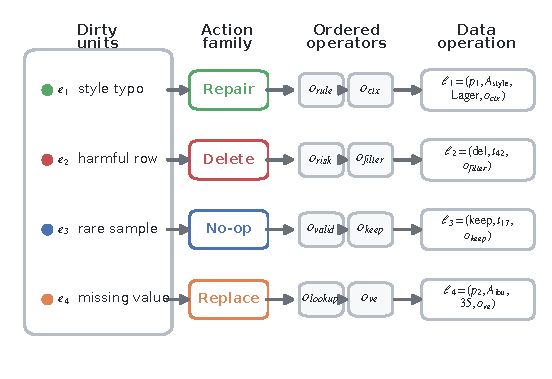
\includegraphics[width=\linewidth]{figures/ddpagent_instance_flow}
  \caption{A cleaning instance of \sys. The agent first selects an action family, then compiles an ordered operator workflow and emits concrete data operations. In the cleaning setting, operators are cleaners, filters, preservers, or value estimators.}
  \Description{A four-row schematic mapping dirty data examples to action families, ordered operators, and concrete data operations.}
  \label{fig:instance}
\end{figure}

This example exposes three challenges for agentic data preparation.

\noindent\textbf{(1) Task demand cannot be inferred from repair correctness alone.}
The same detected issue may require different actions under different downstream metrics, models, budgets, or validation splits. A controller must learn intervention intensity from task feedback instead of from a fixed ordering of suspicious cells.

\noindent\textbf{(2) Action allocation and operator execution live at different granularities.}
Choosing \repair, \deleteop, \replaceop, or \noop specifies the intent of a preparation decision, but it does not determine which rules, contextual signals, estimators, or filters should be ordered into a workflow, nor which concrete value update or row operation should be emitted.

\noindent\textbf{(3) Feedback must govern both regimes and operators.}
A prepared dataset should be treated as a candidate version. Validation may accept selective execution, roll back to \noop, or promote \fullops. The same feedback should also update which actions and operators are trusted later, without requiring new manual labels only to train the allocation policy.

\sys uses a controller and executor loop to address these challenges. An action family captures the semantic intent of an intervention, such as \noop, \repair, \deleteop, or \replaceop. An operator is an executable procedure under that intent, such as a contextual cleaner, a rule-based repairer, a value-estimation routine, or a filtering operator. The controller allocates action families according to task demand. The executor grounds each selected action as an ordered operator workflow and materializes the resulting data operations. Downstream validation selects the final governance regime and feeds utility back to the controller. The current cleaning instantiation uses a learned action allocator trained with zero additional human ground-truth acquisition. In this paper, zero-new-label training means that the policy can use existing operator outputs, cached cleaned versions, and downstream validation feedback, but it does not request new manual labels just to learn which action should be taken.

\sys is a system-level framework rather than a new low-level cleaner. Its contribution is the reusable interface between task demand and operator execution. The system decides whether the task calls for conservative preservation, selective intervention, or full operator execution, then grounds the selected regime in ordered operator workflows and auditable data operations.

We study demand-driven data preparation as governed control over action families, regimes, and reusable operators, and make four contributions.

(1) \textbf{A demand-driven preparation formulation.} We formulate data preparation around task demand rather than around a fixed cleaning objective. The control boundary is an action family or workflow regime. It includes \noop rollback when the data side offers limited measurable gain, selective action allocation when only part of the emitted data operations is useful, and \fullops when broad operator execution is beneficial. This formulation makes preservation and full execution accountable decisions of the agent rather than weak baselines or external competitors.

(2) \textbf{A zero-new-label controller and executor architecture.} We design a two-level agent in which a hierarchical action allocator learns intervention intensity without requesting additional human labels, and an operator-grounded executor compiles the selected action into ordered operator workflows and concrete data operations. The allocator uses downstream utility, budget, detector, model, and execution-history signals. The executor uses action-indexed operator registries so that each action family can own its own compilation network.

(3) \textbf{An operator-grounded governance trace.} \sys records action-level, workflow-level, operator-level, and operation-level provenance for each prepared data version. The trace supports rollback, promotion to \fullops, operator-weight updates, and reuse across future cleaning demands. We evaluate the interface through tabular cleaning, where the implemented action families are preservation, repair, deletion, and replacement.

(4) \textbf{Empirical evidence for demand-driven intervention.} We evaluate five native-error datasets and 40 mixed-error injected settings against fixed cleaners, \sys regimes, and oracle diagnostics. The injected results are reported as per-dataset averages over all eight perturbation rates, and the injected task tables have average cell-level error rate 1.58\%, average record-level error rate 17.78\%, and maximum record-level error rate 50.90\%. The final \sys governance output has the highest average utility among named fixed-cleaner outputs and is first or second on almost all aggregate rows. The selective branch improves or ties \fullops on most rows with average gain 0.0254, while the row where \fullops is better identifies a task that benefits from broad operator execution. The reported rows never fall below \noop after validation. The action traces show that native Tax is deletion-heavy, native Beers and Flights are replacement-heavy, and injected Tax shifts toward a \noop/\deleteop mixture. Together, these cases support the paper's central design choice. Reliable preparation requires choosing the demanded governance regime, compiling the corresponding operator workflow, and materializing the resulting data operations.

\section{Related Work}
\label{sec:related}

We organize prior work by the decision boundary it owns. Fixed cleaning systems decide how to produce a cleaned table. Workflow systems decide how to coordinate multiple operators. Task-aware preparation systems use downstream feedback but usually decide which sample, pipeline, or repair strategy to clean. \sys moves the decision boundary one level higher. It first decides the demanded action family and governance regime, then grounds that decision in reusable operators.

\textbf{Fixed data cleaning operators.}
Classical cleaning work studies how to detect and repair data errors using data-level evidence~\cite{abedjan2016detecting}. Constraint-based systems reason over denial constraints, dependencies, and violation structures to search for consistent repairs~\cite{chu2013holistic,horizon}. Scalable cleansing systems organize rules and operators into executable workflows for large data~\cite{khayyat2015bigdansing}. Probabilistic and Bayesian systems integrate constraints, co-occurrence statistics, and uncertainty to infer likely cell repairs~\cite{rekatsinas2017holoclean,qin2024bclean}, while optimal-transport and conditional-independence approaches target more specific statistical violations~\cite{pirhadi2024otclean}. Learning-based, retrieval-based, and language-model-assisted systems further expand the signal space by using contextual representations, transferred correction evidence, clean corpora, or LLM reasoning~\cite{mahdavi2019raha,mahdavi2019baran,heidari2024lopster,naeem2024retclean,yan2024gidcl,ni2025zeroed}. These methods provide concrete repair, detection, imputation, and filtering operators. Their decision boundary, however, is usually a repaired cell, a repaired table, or a fixed cleaning pipeline optimized by data-level criteria. They do not decide whether the downstream task should preserve, repair, delete, replace, or fully execute operators on a particular unit.

\textbf{Operator coordination and mixed-error workflows.}
Real tables rarely contain a single isolated error type. A repair produced for one attribute may become the source evidence for another operator, and two operators may propose conflicting values for the same target attribute. Existing systems study multi-signal integration, dependency-aware execution, and workflow optimization~\cite{rekatsinas2017holoclean,khayyat2015bigdansing,horizon,siddiqi2024saga,mohammed2025stepbystep}. This line of work motivates the executor in \sys. Operators should expose their scope, target, cost, output, and provenance so that a workflow can reason about dependencies and conflicts. The remaining gap is the control boundary above the workflow. Coordinating cleaners answers how a repair workflow should run once repair is desired. It does not by itself answer whether the task demands repair at all, or whether deletion, low-cost replacement, preservation, rollback, or full operator execution is the better governance decision.

\textbf{Task-aware data preparation.}
Another line connects data cleaning or preparation with downstream machine learning. ActiveClean prioritizes records for cleaning under model training feedback~\cite{krishnan2016activeclean}, BoostClean searches over detector and repair combinations for model performance~\cite{krishnan2017boostclean}, and GoodCore studies data-efficient learning over incomplete data~\cite{goodcore}. CPClean focuses on certain predictions over incomplete information~\cite{karlas2020cpclean}. Context-aware and pipeline-level systems construct or optimize preparation plans for ML tasks~\cite{ctxpipe2024,siddiqi2024saga,mohammed2025stepbystep}. These systems establish the central premise that downstream utility should guide data preparation. Their controls are nevertheless different from ours. They usually clean selected records, choose a pipeline, optimize an order, or target a specific prediction setting. \sys makes the per-unit action family explicit and treats \noop rollback, selective execution, and \fullops promotion as governed outcomes rather than as external baselines.

\textbf{Data-centric AI and extensible preparation actions.}
Data-centric AI argues that improving data can be as important as changing models~\cite{jarrahi2023datacentric,jakubik2024datacentric}, and data-quality-aware MLOps emphasizes that data interventions must be tracked and evaluated in operational ML workflows~\cite{renggli2020snoopy}. Related preparation operators include uncertainty-driven imputation and imputation-order optimization~\cite{wang2024nomi,zhang2025thinktwice}, data valuation and selection~\cite{loizou2025cdash,zhang2025diversity}, and augmentation operators such as mixup and CutMix~\cite{zhang2018mixup,yun2019cutmix}. We do not evaluate these non-cleaning actions in this paper. They clarify the intended boundary of \sys. A data-governance agent should register new action families only when their units, admissible operators, costs, outputs, and provenance are explicit. The evaluated instance is tabular cleaning, where this boundary is instantiated by preservation, repair, deletion, and replacement.

\section{Problem Formulation}
\label{sec:problem}

We formalize the layer that sits between a downstream task and a library of preparation operators. Let $D$ be a dirty training dataset for task $T$ with evaluation metric $U$. The user or task interface may also provide a candidate model set $\mathcal{M}$, such as random forest, SVM, gradient boosting, or a task-specific estimator. A data profiler, detector, cached prepared version, or prior workflow output produces candidate preparation units $E=\{e_1,\ldots,e_n\}$. A unit can be a cell, a row, a feature group, or a structured violation. In the cleaning instance, it is usually a detected cell-level error. The agent observes a state $s_i$ for each unit, chooses an action family $a_i$, and asks an executor to realize the selected family by ordering operators and emitting concrete data operations. The output is a workflow $W$, a prepared dataset $D_W$, and a provenance trace $\tau_W$.

For example, in the Hospitals task used later, $T$ is measure-code classification, $U$ is accuracy, $E$ contains candidate cells or violations obtained from detectors and cached cleaning outputs, and $\mathcal{A}$ contains preservation, repair, deletion, and replacement. In the Tax-10K task, $T$ is rate regression on a clustered 10K subset, so a suspicious record may be more useful as a deletion candidate than as an individual cell repair. The formulation below keeps both cases in the same interface. The task demand changes, while the allocator and executor still communicate through action families and operator registries.

We introduce the interface in the order that information moves through the system. A task demand first specifies what the downstream workflow cares about. The action family then states the intended intervention for a unit. After the selected actions are executed, the governance regime decides which prepared data version should be committed. Operator grounding and the demand-driven policy connect these objects to executable workflows and learned control.

\begin{definition}[Task demand]
A task demand is a tuple
\[
q=(T,U,\mathcal{M},D,E,\mathcal{A},\Omega,B,\mathcal{P}),
\]
where $T$ and $U$ define the downstream task and metric, $\mathcal{M}$ is the optional candidate model set, $E$ is the preparation-unit set, $\mathcal{A}$ is the action-family space, $\Omega=\{\Omega_a\mid a\in\mathcal{A}\}$ is the action-indexed operator registry, $B$ is the human or execution budget, and $\mathcal{P}$ contains policy constraints such as whether deletion is allowed. Evidence sources such as detector scores, rule violations, cached cleaned versions, validation outputs, or prior execution traces are encoded in the state $s_i$. Governance regimes are defined separately because they are commit decisions after execution rather than fields of the user demand.
\end{definition}

The tuple is deliberately wider than a dirty table and a detector output. It makes the downstream objective, candidate models, action space, operator registry, and governance constraints visible before execution. This is necessary because the same suspicious cell can be handled differently when the budget, task metric, or admissible operators change.

\begin{definition}[Action family]
An action family $a\in\mathcal{A}$ denotes the semantic intent of a preparation decision. It is not an executable program. In the cleaning instantiation, the action space is
\[
  \mathcal{A}_{\mathrm{clean}}=\{\noop,\repair,\deleteop,\replaceop\},
\]
corresponding to preservation, correction, removal, and low-cost substitution.
The action space is an interface rather than a closed list. A system can add a new family by specifying its preparation units, state features, admissible operators, cost model, and provenance schema. For example, a data-augmentation family would not reuse the repair operators directly. It would register augmentation operators that expose their generated samples, affected labels or features, cost, and validation feedback through the same $\Omega_a$ interface. We evaluate the cleaning instance, but the controller and executor communicate through this extensible action and operator boundary.
\end{definition}

The action family is local to a preparation unit. A workflow still needs a dataset-level decision after execution, because a selective candidate may fail validation, while a complete all-operator workflow may be better than selective pruning. This motivates a separate regime variable.

\begin{definition}[Governance regime]
A governance regime $\rho\in\mathcal{G}$ denotes the workflow-level decision after action execution and validation. In the current instantiation,
\[
  \mathcal{G}_{\mathrm{clean}}=\{\mathit{rollback},\mathit{selective},\mathit{fullops}\}.
\]
The rollback regime returns the current data version and corresponds to dataset-level \noop when edits do not improve utility. The selective regime commits only the data operations emitted by action-allocated workflows. The \fullops regime commits the complete all-operator workflow output when broad operator application is beneficial.
\end{definition}

A regime says which data version should be committed, but it still does not specify what the executor emits. We first define the operation record that appears in the workflow and provenance trace.

\begin{definition}[Data operation]
A data operation $\ell$ is the auditable edit or preservation record emitted by an action workflow for a preparation unit. It records the selected action family, the scope of affected tuples or cells, the target attribute when applicable, the proposed value when applicable, the originating operator, execution cost, and commit status. In repair or replacement, we write
\[
  \ell=(a,p,A_t,v',o,c_\ell),
\]
where $p$ is the predicate scope, $A_t$ is the target attribute, $v'$ is the candidate value, and $o$ is the operator that generated the value. When the action and cost are clear, we use the shorter form $\ell=(p,A_t,v',o)$. A deletion operation records a scoped removal such as $\ell=(\deleteop,p,o,c_\ell)$, and a \noop operation records intentional preservation of the unit. This object is the unit that can be committed, pruned, rejected, or traced back to an operator.
\end{definition}

With data operations in place, the next definition gives the executor contract that maps an action family to an ordered operator workflow.

\begin{definition}[Operator grounding]
For each action family $a$, $\Omega_a$ denotes the concrete operators that can realize it. Each operator exposes a scope, input requirements, source attributes, target attributes, cost, output type, and provenance fields. The grounding function $g(e_i,a_i,\Omega_{a_i})$ does not choose a single operator. It constructs or reuses an action-specific operator network, orders applicable operators, generates candidate operations $\ell$, and appends accepted operations to workflow $W$.
\end{definition}

Finally, the controller is the policy that chooses among these action families under the task demand.

\begin{definition}[Demand-driven policy]
The allocator is a policy $\pi_\theta(e_i,s_i,q)\rightarrow a_i$ that maps an issue, a task-aware state, and a demand specification to an action family. The policy is demand-driven because the same issue may receive different actions under different downstream metrics, budgets, or operator availability.
\end{definition}

The optimal tuple $(\rho^*,\pi^*,W^*,M^*)$ maximizes downstream utility after execution while accounting for human and execution costs.
\begin{equation}
  \begin{aligned}
  \max_{\rho,\pi,W,M}\quad
  &U(M,T,D_{\rho,\pi,W})\\
  &-\lambda C_{\mathrm{exec}}(\rho,W)-\gamma C_{\mathrm{human}}(\rho,W)\\
  \text{s.t.}\quad
  &\rho\in\mathcal{G},\;\pi\in\Pi,\\
  &W\in\mathcal{W},\;M\in\mathcal{M},
  \end{aligned}
  \label{eq:objective}
\end{equation}
subject to the allowed action space, operator availability, mutual exclusivity for each preparation unit, and any user-specified budget or policy constraints. If $\mathcal{M}$ contains a single model, Equation~\ref{eq:objective} reduces to the fixed-model setting. In the cleaning instantiation, human cost is especially important because ground-truth repair is expensive and often unavailable at deployment time. Zero-new-label action-allocation training corresponds to the regime where the allocator does not request new human labels to learn the policy, even though it may spend computation and reuse existing operator-generated evidence.

This formulation differs from operator-only cleaning. A fixed cleaner directly searches for a repair $D'$ that improves data-level correctness. \sys\ searches over action families, operator realizations, and workflow regimes with respect to downstream utility. Downstream validation adds a governance layer around this objective. When a candidate execution lowers the validation utility relative to the reference data, the final decision can roll back to \noop. When the complete all-operator workflow is consistently better than selective pruning, the system can expose \fullops as the appropriate execution regime. Neither outcome is a failure case. Rollback means that the data side offers limited measurable gain for the current task, while \fullops means that the task benefits from broad operator application.

\section{\sys\ Framework and Execution Loop}
\label{sec:execution}

Figure~\ref{fig:framework} shows the four-block framework. The section follows the execution order of the system. Step~1 converts a downstream request into a typed demand. Step~2 trains an action allocator over the candidate units without requesting new manual labels for policy learning. Step~3 executes the learned actions by indexing into action-specific operator registries, ordering the operators, and committing concrete data operations. Step~4 records action, workflow, operator, and operation provenance and feeds downstream validation back to both the allocator and the operator weights. The bottom feedback edge is downstream validation rather than an independent fifth module. It evaluates each prepared data version and can accept the selective candidate, roll back to the reference data, promote full operator execution, or update the allocation policy with the observed utility change.

\begin{figure*}
  \centering
  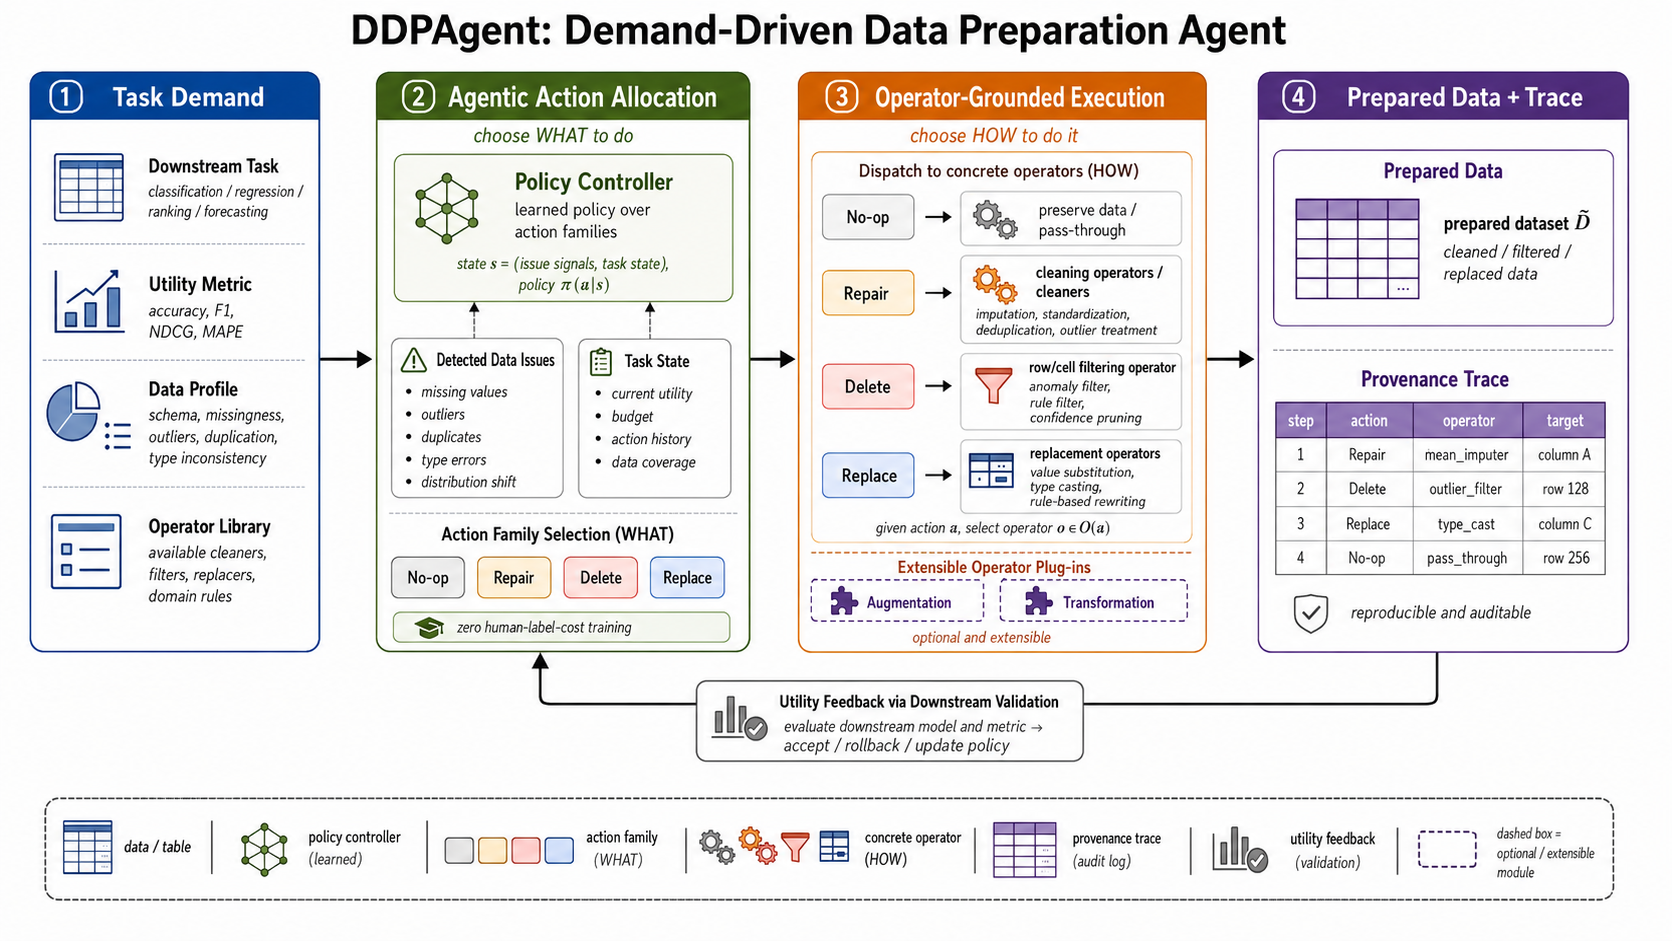
\includegraphics[width=0.98\textwidth]{figures/ddpagentframeworkv0520}
  \caption{\sys framework. A task demand is converted into action-family allocation, grounded as ordered operator workflows, and materialized as prepared data with action, workflow, operator, and operation provenance. The bottom edge denotes downstream validation feedback, which can accept selective execution, roll back to \noop, promote \fullops, or update the allocation policy.}
  \Description{A four-block system diagram with task demand, action allocation, operator-grounded workflow execution, prepared data with provenance trace, and downstream validation feedback.}
  \label{fig:framework}
\end{figure*}

\subsection{Step 1: Demand Specification}

The first step converts a downstream request into the typed demand tuple $q$. This input contract is more specific than a dirty table. It includes the downstream task and target column, the validation metric, optional candidate downstream models, candidate preparation units, action families, action-indexed operator registries, budget, and policy constraints. In the current cleaning instance, the candidate units are detected cells and additional cells suggested by differences between dirty data and cached cleaning outputs. The evidence sources used for state encoding, denoted by $\mathcal{S}$ in the algorithms, include detector confidence, rule violations, feature importance from the downstream model, cached repair values, and execution histories. The operator registry includes cleaning operators, value estimators, row filters, and pass-through operators.

Each operator is registered by a small schema containing source scope, target scope, input requirements, output type, cost, and provenance fields. For example, a repair operator may expose $A_s\rightarrow A_t$, a detector function, and a value generator. A delete operator exposes a row scope and a retention constraint. A replacement operator exposes a candidate-value source and admissible domain. This contract lets the allocator reason over action families without knowing the internal implementation of every operator, and lets the executor later build action-specific operator networks. It is also the extension mechanism of the framework. Adding an action family requires adding $\Omega_a$ and the corresponding state/provenance fields, not rewriting the allocator around one concrete tool. In the experiments, the tuple is produced by configuration and dataset metadata. The method only assumes that later decisions are conditioned on this structured demand.

The tuple also prevents a common ambiguity in tool-using data agents. A request such as ``prepare the hospital table for measure-code prediction'' is not executable until it is grounded into a target column, a validation split, allowed actions, candidate units, and operator registries. Once these fields are explicit, a cleaning operator, a row filter, and a value estimator can all be considered by the same controller without being treated as interchangeable tools.

\subsection{Step 2: Zero-New-Label Action Allocation Training}

The second step trains a task-aware action allocator without requesting additional human ground-truth labels. Zero-new-label here means zero new manual annotation for learning the allocation policy. The allocator may still use computation, detector outputs, cached dirty/cleaned versions, operator-generated candidates, and validation feedback that already exist in the data governance environment. When candidate downstream models are provided, the system first selects or fixes the evaluation model used by the allocator. A practical choice is to prefer models that are both competent on the task and responsive to data preparation, because a model whose metric does not change under any preparation action gives weak reward signals.

Training is cast as a sequential decision problem over $E$. Each candidate unit is represented by a state vector rather than by its raw value alone. In the cleaning instance, the state vector contains local signals such as issue type, column type, detector confidence, feature importance, boundary distance, and column error rate. It also contains global data-quality signals such as sample retention and distributional retention, budget signals such as remaining human budget and remaining issue ratio, and execution-history signals such as whether an operator candidate exists and how similar operators behaved previously. The policy then learns a mapping from state and demand to an action family:
\[
  \pi_\theta(e_i,s_i,q)\rightarrow
  a_i\in\{\noop,\repair,\deleteop,\replaceop\}.
\]
The action family is intentionally coarser than an operator workflow. \repair\ means that a correction is demanded. It does not yet decide which rule, dependency, or contextual cleaners should be ordered, nor which candidate value should be committed. \replaceop\ means that a lower-cost estimate is acceptable. It does not hard-code which lookup or estimator should run first. \deleteop\ means the issue scope is more harmful than useful under the task demand. \noop\ is a first-class decision when the detector is uncertain, the task is tolerant, or intervention would remove useful boundary cases.

The current allocator uses a hierarchical Dueling Double DQN design. Stage 1 performs cost-free triage and selects among \noop, \deleteop, and \emph{enter intervention}. Stage 2 is triggered only for intervention candidates and selects between low-cost replacement and costly repair. This prevents a flat action space from degenerating into always repairing whenever a reference value is available. Each stage has its own value and advantage heads,
\[
Q_j(s,a)=V_j(s)+A_j(s,a)-|\mathcal{A}_j|^{-1}\textstyle\sum_{a'} A_j(s,a'),
\]
where $j\in\{1,2\}$ denotes the stage. Target networks and replay buffers are maintained separately, because Stage 1 mainly learns whether intervention is needed, while Stage 2 learns how much cost the intervention should spend.

The reward combines three signals. A shaping reward gives dense guidance from issue priority, feature importance, detector confidence, deletion risk, and budget slack. A periodic proxy reward measures the change in downstream validation utility after a batch of decisions, subtracting cost for human repair. A terminal reward compares the final prepared candidate against the baseline data version while penalizing lost samples and spent human budget. If the remaining budget is exhausted, repair is automatically downgraded to a zero-cost replacement or \noop action according to policy constraints. This training procedure makes action allocation a task-conditioned controller rather than a fixed ranking of suspicious cells.

Algorithm~\ref{alg:allocation-training} summarizes the training loop. The key point is that the environment is built from existing data versions and operator evidence, not from newly requested manual labels. The allocator observes how candidate actions change downstream validation utility and learns a cost-aware policy over action families.

A typical decision illustrates the two-stage structure. If a candidate unit lies in a low-importance column with weak detector confidence, Stage~1 can select \noop and avoid unnecessary execution. If the unit is high-impact, Stage~1 enters intervention. Stage~2 then chooses \repair when the evidence store contains reliable correction evidence and the remaining budget allows it, or \replaceop when the task can tolerate a lower-cost estimate. This is why the policy is trained over action families rather than concrete cleaners. The allocator learns how much intervention the task demands before the executor orders operators and emits the concrete operation.

\begin{algorithm}[t]
\caption{Zero-New-Label Action Allocation Training}
\label{alg:allocation-training}
\vspace{-1mm}
\small
\begin{algorithmic}[1]
\REQUIRE Demand $q$, dirty data $D$, units $E$, signals $\mathcal{S}$, operators $\Omega$, validation split, episodes $N$
\ENSURE Action allocator $\pi_\theta$
\STATE Build evidence store $\mathcal{C}$ from cached data versions, detector outputs, and operator candidates
\STATE Select or fix downstream evaluator $M\in\mathcal{M}$ for utility $U$
\STATE Initialize two-stage Q networks $Q_1,Q_2$, targets $\bar Q_1,\bar Q_2$, replay buffers $\mathcal{B}_1,\mathcal{B}_2$
\FOR{episode $=1$ to $N$}
    \STATE $D^{(0)}\leftarrow\textsc{SampleVersion}(D,\mathcal{C})$, $B_{\mathit{rem}}\leftarrow B$, and $\tau\leftarrow\emptyset$
    \FOR{each preparation unit $e_i\in E$}
        \STATE $s_i\leftarrow\textsc{Encode}(D^{(t)},e_i,q,\mathcal{S},B_{\mathit{rem}},\tau)$
        \STATE $z_i\leftarrow\textsc{EpsGreedy}(Q_1,s_i,\epsilon)$ over $\{\noop,\deleteop,\mathit{intervene}\}$
        \IF{$z_i=\mathit{intervene}$}
            \STATE $a_i\leftarrow\textsc{EpsGreedy}(Q_2,s_i,\epsilon)$ over $\{\replaceop,\repair\}$
            \IF{$a_i=\repair$ and ($B_{\mathit{rem}}=0$ or \textsc{NoEvidence}$(e_i,\mathcal{C})$)}
                \STATE $a_i\leftarrow\textsc{Downgrade}(\replaceop,\noop,\mathcal{P})$
            \ENDIF
        \ELSE
            \STATE $a_i\leftarrow z_i$
        \ENDIF
        \STATE $(D^{(t+1)},c_i,\tau_i)\leftarrow\textsc{SimulateOrReplay}(D^{(t)},e_i,a_i,\Omega_{a_i},\mathcal{C})$
        \STATE $r_i\leftarrow\textsc{ShapeReward}(s_i,a_i,c_i,q)$ and store transition in $\mathcal{B}_1$ or $\mathcal{B}_2$
        \STATE Periodically add proxy reward $\Delta U(M,T,D^{(t+1)})-\lambda c_i$
        \STATE Update $Q_1,Q_2$ from replay buffers and softly update $\bar Q_1,\bar Q_2$
    \ENDFOR
    \STATE Add terminal reward from $U(M,T,D^{(T)})$, retention, and spent budget
    \STATE Save $\theta$ if validation utility improves, breaking ties by lower human cost
\ENDFOR
\STATE \textbf{return} best historical allocator $\pi_\theta$
\end{algorithmic}
\vspace{-1mm}
\end{algorithm}

\subsection{Step 3: Inference-Time Action Execution}

At inference time, the learned allocator assigns action families to candidate units for a new demand. The executor then grounds each action through an action-specific operator network $G_a$. In the cleaning instantiation, \noop\ is grounded as traceable pass-through, \repair\ as an ordered repair workflow, \deleteop\ as row- or cell-scope filtering, and \replaceop\ as an ordered value-estimation workflow. This division is the core of the data governance agent. The allocator decides what action the task demands, while the executor decides how the selected action is realized by ordering the current operator pool and committing concrete operations.

The executor also supports workflow-level regimes. The default regime is selective execution, where only the operations emitted by action-allocated workflows are committed. The \noop regime is a conservative rollback path selected when validation shows that editing does not improve the current task. The \fullops regime materializes the complete all-operator workflow output without selective pruning. It is useful when the downstream task benefits from broad application of the available operator pool. Reporting these regimes separately is not a comparison between \sys and external alternatives. It exposes the three outcomes that a data governance agent may choose under different data states.

Algorithm~\ref{alg:operator-execution} gives the inference procedure. The policy only selects action families. The executor then indexes into the corresponding operator registry, builds an action-specific operator graph, orders applicable operators, searches executable operations under that graph, and lets downstream validation choose the final governance regime.

\begin{algorithm}[t]
\caption{Inference-Time Action-Workflow Execution}
\label{alg:operator-execution}
\vspace{-1mm}
\small
\begin{algorithmic}[1]
\REQUIRE Demand $q$, data $D$, units $E$, allocator $\pi_\theta$, operator registries $\Omega$, validator $(M,U)$
\ENSURE Prepared data $D_{\rho}$, workflow $W_{\rho}$, provenance trace $\tau_{\rho}$
\STATE $D_{\mathit{sel}}\leftarrow D$, $W_{\mathit{sel}}\leftarrow\emptyset$, and $\tau_{\mathit{sel}}\leftarrow\emptyset$
\STATE $D_{\mathit{full}}\leftarrow\textsc{ApplyAllOperators}(D,\Omega)$ and $D_{\mathit{noop}}\leftarrow D$
\FOR{each preparation unit $e_i\in E$}
    \STATE $s_i\leftarrow\textsc{Encode}(D_{\mathit{sel}},e_i,q,\mathcal{S},B,\tau_{\mathit{sel}})$
    \STATE $a_i\leftarrow\pi_\theta(e_i,s_i,q)$
    \STATE $G_{a_i}\leftarrow\textsc{BuildOperatorGraph}(\Omega_{a_i},D_{\mathit{sel}},e_i,\tau_{\mathit{sel}})$
    \IF{$a_i=\noop$}
        \STATE Record pass-through decision for $e_i$ in $\tau_{\mathit{sel}}$
    \ELSE
        \STATE $\mathcal{K}_i\leftarrow\textsc{GenerateCandidates}(G_{a_i},D_{\mathit{sel}},e_i)$
        \STATE $\mathcal{O}_i\leftarrow\textsc{SearchOperations}(\mathcal{K}_i,G_{a_i},q)$
        \STATE $(D_{\mathit{sel}},W_{\mathit{sel}},\tau_{\mathit{sel}})\leftarrow\textsc{CommitIfImproves}(\mathcal{O}_i,D_{\mathit{sel}},W_{\mathit{sel}},\tau_{\mathit{sel}})$
        \STATE Update operator weights from accepted, rejected, and conflicting candidates
    \ENDIF
\ENDFOR
\STATE $u_{\mathit{rollback}}\leftarrow U(M,T,D_{\mathit{noop}})$ and $u_{\mathit{selective}}\leftarrow U(M,T,D_{\mathit{sel}})$
\STATE $u_{\mathit{fullops}}\leftarrow U(M,T,D_{\mathit{full}})$
\STATE $\rho\leftarrow\arg\max_{\rho\in\{\mathit{rollback},\mathit{selective},\mathit{fullops}\}} u_{\rho}$
\STATE \textbf{return} data, workflow, and trace associated with $\rho$
\end{algorithmic}
\vspace{-1mm}
\end{algorithm}

Each action family can have its own compilation network. For \repair, the network is built over heterogeneous cleaning signals. Each repair operator is represented as $o=[\mathrm{detect}_o,f_o]$ from $A_s$ to $A_t$, where $A_s$ is the source scope, $A_t$ is the target scope, $\mathrm{detect}_o$ estimates whether a tuple remains erroneous, and $f_o$ generates candidate values. The executor first separates single-scope operators from multi-attribute operators. Single-scope operators can run as a parallel preprocessing layer. Multi-attribute operators form a dependency graph. If $A_{t_i}\cap A_{s_j}\neq\emptyset$, then the output of $o_i$ can affect the evidence used by $o_j$. If two operators share the same target scope, their repairs can conflict. Cycles are merged into a block, independent blocks are scheduled by topological level, and operators inside a block are ordered by their current weights.

Within a repair block, the executor generates candidate operations rather than immediately editing the table. For low-quality tuples, it collects source-attribute values as predicates that locate the affected records. From high-quality tuples, cached repaired data, or external knowledge, it collects candidate target values. A candidate repair operation has the form $\ell=(\repair,p,A_t,v',o,c_\ell)$, where $p$ is the predicate scope, $v'$ is the proposed value, $o$ is the originating operator, and $c_\ell$ is its cost. For example, if an action selects \repair for a violation involving $A_s\rightarrow A_t$, dependency and context signals may propose different values for $A_t$ under the same predicate $p$. The search procedure evaluates candidates by the weighted residual detector score plus modification cost. It applies the best candidate only if it reduces the block objective, updates the data and quality scores, removes redundant candidates with the same predicate or target, and stops when no candidate further improves the block. This gives the \repair\ action a concrete compilation path through operator association, block construction, operator ordering, candidate generation, repair search, and weight update. The committed output is not a cleaner name alone. It is an operation such as assigning a repaired value to a target attribute or removing a tuple under a recorded predicate.

The other action families use the same grounding interface with different operator networks. \replaceop\ orders lower-cost estimators, such as dependency-based lookup, neighborhood estimation, cached cleaned-value lookup, or domain-constrained imputation, when exact repair is not demanded or not available. \deleteop\ materializes a row- or cell-scope filtering operation subject to retention constraints, so that one uncertain signal is not enough to remove a row. \noop\ records an intentional preservation decision rather than silently skipping the unit. The current evaluation instantiates these four cleaning actions. The important interface property is that execution is action-specific and workflow-oriented rather than cleaner-specific.

\subsection{Step 4: Provenance and Feedback}

The fourth step records the action, workflow, operator, and operation trace and feeds the observed utility back to both the allocator and the operator networks. The trace stores the preparation-unit identifier, selected action family, stage decisions, ordered operator workflow, operation identifier $\ell$, source scope, target scope, predicate, dirty value, candidate value, final value, input data version, output data version, execution cost, and validation delta. In the current implementation this information is materialized as a decision log, a deferred repair plan, a repair-source log, an operator execution trace, and a run-level metric file.

For a repair action, provenance is produced at four granularities. The action record explains why the unit entered \repair\ rather than \noop, \deleteop, or \replaceop. The workflow record stores the ordered operators and the dependency block that produced the candidates. The operator record identifies the source-target dependency, such as $A_s\rightarrow A_t$, and the signal that generated a candidate. The operation record stores the concrete $\ell$, its predicate scope, target attribute, candidate value, originating operator, and status. The status indicates whether the candidate was committed, pruned as redundant, rejected because it did not reduce the block objective, or overwritten by a higher-weight candidate. The operation-level record makes multi-cleaner execution auditable by exposing the final value, selected action family, operator order, materialized data operation, and discarded competing candidates.

Feedback is used at two levels. At the action level, downstream validation supplies the reward signal that makes the allocator prefer high-utility actions under the current task. If the prepared candidate lowers validation utility relative to the reference data, rollback selects \noop\ at the dataset level even when many cell-level edits look plausible. If a candidate improves the metric, the corresponding action decisions receive positive evidence. At the operator level, the same trace updates the priority of signals inside an action family. Operators whose candidate fixes survive conflict resolution and improve the block or downstream objective receive higher weights in later repair blocks. Operators that produce overwritten, conflicting, or harmful candidates are down-weighted or skipped in later candidate generation. Feedback is not only a final accept/reject gate. It changes both the action preference learned by the policy and the operator preference used by the executor when a later unit is assigned to the same action family.

This mechanism is the governance layer of \sys. The system outputs a data version together with a reproducible action, workflow, operator, and operation history and a recoverable feedback path. The same trace can support audit, rollback, and reuse. If a future task has a similar demand tuple, the allocator can reuse action-level evidence, and the executor can initialize operator ordering and weights from previously successful action networks.

\subsection{Governance Decisions Exposed by the Loop}

The previous four steps define the execution mechanism. They also expose the decisions that a data-governance agent must report to users and to later workflow runs. These decisions are not extra assumptions. They are the operational consequences of separating task demand, action allocation, operator grounding, and validation feedback.

\textbf{Demand control is separated from operator execution.}
Action allocation and operator execution should not be collapsed. Data cleaning research has produced many specialized repair, imputation, filtering, and consistency-checking operators. A scalable preparation agent should keep these methods as reusable operators and learn a control layer that decides whether the current task demands them. This also avoids an important failure mode of tool-using agents. Once the agent chooses a concrete cleaner too early, it has already committed to the cleaner's objective rather than the downstream task objective.

\textbf{Preservation and full execution are accountable regimes.}
\noop\ should be modeled as an explicit action. In an operator-only pipeline, preservation is usually treated as the absence of a decision. In a governance agent, it is a positive decision. The system may preserve a suspicious value because the detector is uncertain, the model is tolerant, or the sample carries useful distributional information. \fullops has the symmetric meaning at the workflow level. It records that the task benefits from broad operator application, so selective pruning is unnecessary or harmful for that demand. These two regimes define the conservative and intensive ends of the same governance space. Neither should be interpreted as an external baseline that defeats the agent.

\textbf{Action families define the extension boundary.}
The current instantiation uses \noop, \repair, \deleteop, and \replaceop because the experiments focus on cleaning. The key requirement is not that every cleaner be redesigned, but that each operator exposes its scope, cost, output data version, and validation feedback. The same boundary can host non-cleaning preparation families only after they are made explicit in the demand tuple. For instance, a future augmentation family would need its own unit definition, candidate generator, label or feature scope, cost, and provenance fields before the allocator can choose it. Under this view, traditional cleaning methods are not superseded by the agent. They become governed operators under task-aware action families.

\textbf{Preparation is evaluated as a governed workflow.}
Cell-level repair accuracy remains useful for diagnosing an operator, but it is insufficient for an autonomous preparation agent. The system should be judged by downstream utility, execution cost, human-label cost, traceability, and the ability to recover from harmful interventions. This boundary motivates the native-error, injected-error, and feedback analyses in Section~\ref{sec:evaluation}. It also explains why the evaluation includes diagnostic controls such as full repair and oracle deletion. These controls test whether aggressive correctness-oriented interventions help the downstream workflow.

\section{Experimental Evaluation}
\label{sec:evaluation}

The current implementation instantiates \sys\ for tabular cleaning. Candidate errors are obtained from available detectors and cached cleaning outputs. The action allocator is trained without additional human labels and predicts action families for the detected issues. The executor compiles selected actions into ordered cleaning workflows, emits data operations, and produces a prepared table. Downstream validation then evaluates the model on a fixed split and selects among conservative rollback, selective execution, and full operator execution according to task utility. The evaluation focuses on whether the control-and-execution design identifies the demanded governance regime, rather than cell-level repair accuracy alone.

We ask three questions. \textbf{RQ1} asks whether the final governance output competes with fixed cleaning methods on native errors. \textbf{RQ2} asks whether the same control loop remains useful under controlled mixed-error injection rather than only on the native data. \textbf{RQ3} asks when the agent should preserve, selectively intervene, or fully apply operators, and whether action traces explain these regimes.

\subsection{Experimental Setup}

The evaluation uses five datasets with native errors and the same five datasets under mixed-error injection. Table~\ref{tab:datasets} lists the task settings. Following standard cleaning reports, C\% and R\% denote cell-level and record-level error rates on the task rows. M, T, F, and V abbreviate missing values, typos/outliers, format inconsistencies, and attribute-dependency violations. The large Tax case is evaluated on a clustered 10K subset rather than a random sample, so records sharing key-like structure remain together. The Hospitals target is measure-code classification. This avoids the saturated ownership-label split and gives cleaning actions a measurable downstream effect. The reported experiments use a singleton downstream model per dataset. In this setting, the candidate-model interface in Section~\ref{sec:problem} is exercised as fixed-model task demand rather than as model selection.

\begin{table}[t]
  \caption{Summary of datasets and downstream tasks. C and R denote classification and regression.}
  \label{tab:datasets}
  \centering
  \small
  \begin{tabular}{@{}lrrrrll@{}}
    \toprule
    Data & Rows & Col. & C\% & R\% & Err. & Task \\
    \midrule
    Beers & 2.4K & 10 & 13.94 & 100.00 & M/F/V & C-style \\
    Flights & 1.1K & 7 & 15.45 & 56.42 & M/F/V & C-delay \\
    Hospitals & 1.0K & 19 & 2.68 & 40.70 & T/V & C-measure \\
    Rayyan & 642 & 11 & 10.25 & 84.58 & M/T/F/V & C-lang. \\
    Tax-10K & 10K & 15 & 0.11 & 1.65 & T/F/V & R-rate \\
    \bottomrule
  \end{tabular}
\end{table}

We evaluate fixed cleaning baselines, deployable \sys regimes, and oracle diagnostic references. For each fixed cleaner, we train and evaluate the same downstream model directly on the cleaned table produced by that method. This protocol compares data preparation outputs rather than internal cell-level objectives. We also report two internal governance regimes of \sys. The \noop regime preserves the dirty input and is selected when validation indicates limited measurable data-side gain. The \fullops regime bypasses selective pruning, directly takes the complete all-operator workflow output from the execution substrate, and trains the downstream model on that full output. \fullops answers when the task demands broad operator application, while selective \sys tests whether task-conditioned action allocation should commit only the operations emitted by selected workflows. Oracle deletion removes rows containing known true errors and tests whether aggressive authenticity improvement helps after sample loss. Full ground-truth repair replaces all known erroneous cells with clean values and tests whether maximum cell-level correctness is aligned with task utility. These oracle diagnostics use clean-reference information that a practical system does not have at deployment time, so they are diagnostic references rather than ordinary cleaning baselines or \sys operating modes. The reported native setting contains 45 baseline, regime, and reference evaluations. The reported injected setting contains 40 preparation cases and 360 baseline, regime, and reference evaluations.

Table~\ref{tab:baseline-taxonomy} organizes the evaluated methods by the decision they are allowed to make before downstream evaluation. This taxonomy is important for interpreting the results. A fixed cleaner is allowed to output one cleaned table. A \sys regime is allowed to decide which prepared data version should be committed. An oracle diagnostic is allowed to use clean-reference information that is unavailable at deployment time. The table also records the evidence each method uses, the action or regime it can express, and its role in the evaluation.

\begin{table*}[t]
  \caption{Taxonomy of evaluated methods by decision boundary. ``Boundary'' describes what the method is allowed to decide. ``Coverage'' lists the action family or workflow regime it can express. ``Oracle'' marks clean-reference access.}
  \label{tab:baseline-taxonomy}
  \centering
  \small
  \begin{tabular}{@{}p{0.08\textwidth}p{0.115\textwidth}p{0.14\textwidth}p{0.16\textwidth}p{0.13\textwidth}p{0.145\textwidth}p{0.05\textwidth}@{}}
    \toprule
    Family & Method & Boundary & Evidence & Coverage & Evaluation role & Oracle \\
    \midrule
    Fixed cleaner & Baran~\cite{mahdavi2019baran} & cell repair & transferred cell context & repair & contextual repair baseline & No \\
    Fixed cleaner & BigDansing~\cite{khayyat2015bigdansing} & cleansing workflow & rule/operator execution & repair/filter & workflow baseline & No \\
    Fixed cleaner & Holistic~\cite{chu2013holistic} & repair set & denial constraints & repair & constraint baseline & No \\
    Fixed cleaner & HoloClean~\cite{rekatsinas2017holoclean} & probabilistic repair & constraints and co-occurrence & repair & probabilistic baseline & No \\
    Fixed cleaner & Horizon~\cite{horizon} & dependency plan & discovered dependencies & repair & dependency baseline & No \\
    DDP regime & \sys & unit action plus data-version regime & downstream demand and workflow trace & multi-action & final governed output & No \\
    DDP regime & \noop & committed data version & dirty input and validation feedback & rollback & conservative regime & No \\
    DDP regime & \fullops & committed data version & all-operator workflow and validation feedback & full execute & intensive regime & No \\
    Oracle diag. & OracleDel & true-error row deletion & clean-reference error rows & delete & deletion diagnostic & Yes \\
    Oracle diag. & GTRepair & true-cell repair & clean-reference erroneous cells & repair & correctness diagnostic & Yes \\
    \bottomrule
  \end{tabular}
\end{table*}

For injected data, we follow the mixed-error construction used in data cleaning benchmarks. For each dataset, non-key attributes and applicable constraints are independently perturbed with typographical or outlier edits, missing values, and rule-violation values. We use eight cell- or rule-level injection rates between $0.25\%$ and $2.0\%$. Dataset names with $^*$ denote arithmetic means over these eight injected settings. No dataset is reported at a single favorable injection level. Since a tuple may contain several attributes and participate in multiple constraints, record-level error rates can be much higher than the nominal cell- or rule-level rate. Table~\ref{tab:injection-strength} reports the measured cell-level and record-level intensity against the clean reference after applying the same task filtering and subsetting as the evaluation. Across the 40 reported injected task tables, the average cell-level error rate is 1.58\%, the average record-level error rate is 17.78\%, and the hardest setting reaches 50.90\% erroneous rows. The resulting 40 cases require the allocator to avoid unnecessary changes under mild corruption and select demanded interventions when mixed errors affect downstream utility.

\begin{table}[t]
  \caption{Cell-level and record-level intensity of the injected task tables. Each row summarizes the eight injected settings used for that dataset's aggregate injected result. Tax is measured on the clustered 10K subset.}
  \label{tab:injection-strength}
  \centering
  \small
  \begin{tabular}{@{}lrrrrr@{}}
    \toprule
    Data & Ver. & Avg. C\% & Range C\% & Avg. R\% & Range R\% \\
    \midrule
    Beers & 8 & 1.30 & 0.62 to 1.98 & 12.50 & 6.18 to 17.93 \\
    Flights & 8 & 1.89 & 0.44 to 3.35 & 11.14 & 3.03 to 19.23 \\
    Hospitals & 8 & 1.95 & 0.41 to 3.47 & 31.00 & 8.30 to 50.90 \\
    Rayyan & 8 & 0.88 & 0.42 to 1.34 & 9.72 & 4.90 to 14.20 \\
    Tax-10K & 8 & 1.87 & 0.45 to 3.19 & 24.55 & 6.40 to 40.15 \\
    \midrule
    Mean & 40 & 1.58 & 0.41 to 3.47 & 17.78 & 3.03 to 50.90 \\
    \bottomrule
  \end{tabular}
\end{table}

\subsection{Performance on Native Errors}
\label{sec:native-results}

Table~\ref{tab:baseline-cleaners} compares the final \sys governance output with fixed cleaning outputs. The \sys column reports the validation-selected regime among conservative \noop rollback, selective action allocation, and \fullops execution. Table~\ref{tab:ablation} separates these regimes. The values are downstream task utilities after training on each prepared table. Accuracy is used for classification and $R^2$ for Tax regression, and higher is better. Across the table, \sys has the highest mean utility among the named fixed cleaners (0.5372) and is ranked first or second on almost every row, with Hospitals$^*$ as the only third-place case. The best and second-best values in each row are marked in \best{red} and \runner{blue}, respectively, with ties included.

On native errors, \sys is best among fixed cleaned outputs on Beers, Flights, and Hospitals, and second on Rayyan and Tax-10K. The gains over the strongest fixed cleaner are 0.0122 on Beers, 0.0239 on Flights, and 0.0167 on Hospitals, corresponding to relative improvements of 6.8\%, 2.5\%, and 2.0\%. The two second-place cases are also informative. \sys is only 0.0006 below BigDansing on Tax-10K, but 0.0279 below Holistic on Rayyan, where a fixed constraint-oriented output is better aligned with the language-classification target. This pattern is more useful than a simple win count. On Flights, fixed cleaning outputs vary widely. Baran remains close to \sys, but HoloClean and Horizon reduce downstream utility by 0.7400 and 0.1884 relative to \sys. A high-quality cell repair method is not automatically aligned with the task metric.

\textbf{Finding 1. Native preparation is not monotone in cleaning strength.}
Native errors expose a non-monotonic preparation effect. Running a stronger cleaner or more complete workflow does not necessarily improve downstream utility. In Table~\ref{tab:ablation}, the selective policy improves over \fullops by 0.1194 on Flights, 0.0313 on Hospitals, and 0.0267 on Rayyan, while tying it on Beers and Tax-10K. The same table shows that \sys matches \noop on Flights, Hospitals, and Rayyan, indicating that validation sometimes prefers preservation after evaluating a candidate execution. These outcomes are operating-regime decisions, not failures. Matching \noop means that the system found no measurable benefit from committing edits under the current split and metric. Matching or using \fullops means that full operator application is the demanded regime. The target is not maximum edit distance from the dirty table, nor maximum agreement with one cleaning objective. The target is a task-conditioned intervention policy that can be conservative, selective, or intensive.

\begin{table}[t]
  \caption{Comparison with fixed baseline cleaning methods. The \sys column reports the final governance output selected among \noop rollback, selective allocation, and \fullops execution. When a fixed cleaner does not produce an applicable output for a row, we report the corresponding \noop utility as a conservative fallback. Injected rows follow the aggregation protocol in Section~\ref{sec:evaluation}. \best{Red} and \runner{blue} mark the best and second-best downstream utilities in each row, with ties included.}
  \label{tab:baseline-cleaners}
  \centering
  \small
  \setlength{\tabcolsep}{4.5pt}
  \begin{tabular}{@{}lrrrrrr@{}}
    \toprule
    Data & \sys & Baran & BigD. & Hol. & HoloC. & Horiz. \\
    \midrule
    Beers & \best{0.1929} & \runner{0.1807} & 0.1607 & 0.1526 & 0.1511 & 0.1540 \\
    Flights & \best{0.9854} & \runner{0.9615} & 0.9297 & 0.9312 & 0.2454 & 0.7970 \\
    Hospitals & \best{0.8665} & 0.8392 & 0.8075 & 0.8002 & \runner{0.8498} & 0.8457 \\
    Rayyan & \runner{0.1538} & 0.1183 & 0.1205 & \best{0.1817} & 0.0685 & 0.0825 \\
    Tax-10K & \runner{0.5756} & 0.5753 & \best{0.5762} & 0.5751 & 0.4720 & 0.3294 \\
    Beers$^*$ & \best{0.1821} & 0.1728 & 0.1720 & \runner{0.1736} & 0.1724 & 0.1718 \\
    Flights$^*$ & \best{1.0000} & 0.9357 & 0.9910 & \runner{0.9923} & 0.2706 & 0.9099 \\
    Hospitals$^*$ & 0.8571 & 0.8532 & \runner{0.8583} & \best{0.8655} & 0.8460 & 0.7858 \\
    Rayyan$^*$ & \runner{0.1700} & 0.1489 & 0.1214 & \best{0.1889} & 0.0395 & 0.1377 \\
    Tax-10K$^*$ & \best{0.3883} & \runner{0.3414} & -6.5793 & -1.6333 & -5.6384 & 0.1318 \\
    \bottomrule
  \end{tabular}
\end{table}

\subsection{Performance on Injected Errors}
\label{sec:injected-results}

The injected aggregate rows in Table~\ref{tab:baseline-cleaners} use the perturbation protocol and record-level intensities reported in Table~\ref{tab:injection-strength}. They test whether the action allocator remains useful when the error distribution is controlled but heterogeneous. \sys is best on Beers$^*$, Flights$^*$, and Tax-10K$^*$, with relative gains of 4.9\%, 0.8\%, and 13.7\% over the strongest fixed cleaner on those rows. On Rayyan$^*$, the final system promotes \fullops and becomes second, 0.0189 below Holistic. On Hospitals$^*$, \sys is 0.0084 below Holistic and 0.0012 below BigDansing, showing a concrete boundary where a fixed cleaner remains slightly better under the complete all-rate average. The Tax-10K$^*$ row is particularly important because several fixed cleaned outputs degrade the regression utility sharply, while \sys preserves a positive utility close to the stable references. This supports the demand-driven view. A governance agent is useful when it edits helpful cells and when it avoids committing to an operator whose repairs are harmful for the current task.

The injected rows also show the boundary of the current implementation. Holistic is strongest on Hospitals$^*$ and Rayyan$^*$, and \fullops is strongest among the reported \sys regimes on Rayyan$^*$ in Table~\ref{tab:ablation}. When one fixed cleaning workflow or the complete all-operator workflow is consistently well aligned with a task and error distribution, the executor should be able to reuse it without forcing selective pruning. The contribution of \sys is the control interface that can select, skip, roll back, or escalate to full operator execution under downstream feedback rather than claiming that one learned selective policy dominates every fixed cleaner.

\textbf{Finding 2. Mixed errors make operator choice a governance problem.}
Mixed-error injection shows why a governance agent needs to handle heterogeneous operator effects. Across the 40 injected settings, \sys reaches or exceeds the best fixed cleaning output in 21 cases, improves over \noop in 17 cases, and triggers rollback in 18 cases. The action traces explain this split. On injected Beers, the allocator uses a repair/replace-heavy mix with 44.7\% \repair and 48.6\% \replaceop. On injected Rayyan, \replaceop dominates at 60.3\%. On injected Tax, the policy shifts toward 37.1\% \noop and 36.5\% \deleteop. Mixed errors do not demand a uniform cleaning intensity. Some tasks need value-level correction, some need low-cost replacement, and some benefit from preservation or removal. This result supports the action-family abstraction in Section~\ref{sec:execution}. Mixed errors should not force the system to trust a single cleaner globally, because different corruption patterns and downstream tasks demand different intervention families.

\subsection{Action Allocation and Feedback Analysis}

Table~\ref{tab:ablation} separates three \sys governance regimes from diagnostic controls. \noop is the conservative rollback regime. \fullops is the intensive regime that commits the complete all-operator workflow output. \syssel reports the selective action-allocation branch before \noop rollback or \fullops promotion. OracleDel deletes rows containing known true errors, and GTRepair repairs all known erroneous cells with clean values. These two use clean-reference information and are diagnostic controls rather than deployable baselines. When OracleDel has no applicable deletion output for a row, the table reports the \noop utility. The table is not a fixed-cleaner comparison. It explains when the data governance agent should preserve, selectively intervene, fully apply operators, delete by oracle knowledge, or repair by oracle knowledge.

\begin{table}[t]
  \caption{\sys operating regimes and diagnostic comparison. \noop is the conservative rollback regime, \fullops is the full operator-execution regime, and Sel. is the selective action-allocation branch before rollback or \fullops promotion. OracleDel and GTRepair use clean-reference information and are included only to interpret action choices. \best{Red} and \runner{blue} mark the best and second-best values in each row.}
  \label{tab:ablation}
  \centering
  \small
  \begin{tabular}{@{}lrrrrr@{}}
    \toprule
    Data & OracleDel & \fullops & Sel. & GTRepair & \noop \\
    \midrule
    Beers & 0.1511 & \best{0.1929} & \best{0.1929} & \runner{0.1901} & 0.1511 \\
    Flights & 0.9391 & 0.8660 & \runner{0.9854} & \best{1.0000} & \runner{0.9854} \\
    Hospitals & 0.7907 & 0.8352 & \best{0.8665} & \runner{0.8456} & \best{0.8665} \\
    Rayyan & 0.1282 & 0.1271 & \runner{0.1538} & \best{0.1540} & \runner{0.1538} \\
    Tax-10K & \runner{0.5755} & \best{0.5756} & \best{0.5756} & \runner{0.5755} & 0.5751 \\
    Beers$^*$ & 0.1724 & \runner{0.1790} & \best{0.1821} & 0.1773 & 0.1724 \\
    Flights$^*$ & \runner{0.9968} & 0.9027 & \best{1.0000} & \best{1.0000} & \best{1.0000} \\
    Hospitals$^*$ & 0.8125 & 0.8413 & \best{0.8571} & 0.8510 & \runner{0.8564} \\
    Rayyan$^*$ & 0.1104 & \best{0.1700} & 0.1278 & \runner{0.1414} & 0.1241 \\
    Tax-10K$^*$ & 0.3878 & 0.3861 & \best{0.3883} & 0.3881 & \runner{0.3882} \\
    \bottomrule
  \end{tabular}
\end{table}

\begin{figure}[t]
  \centering
  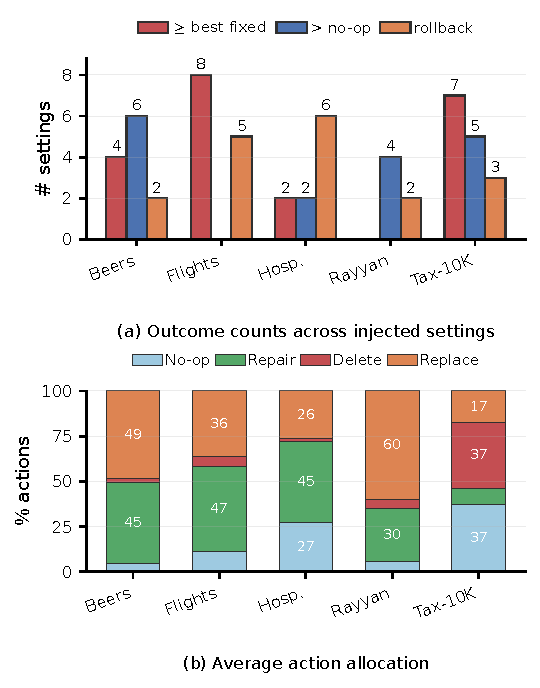
\includegraphics[width=\linewidth]{figures/ddpagent_selected_evidence}
  \caption{Injected-case behavior of \sys across the five reported datasets. Panel (a) counts, out of eight injected settings per dataset, when \sys reaches or exceeds the best fixed cleaning output, improves over \noop, or rolls back a harmful candidate. Panel (b) reports the average action allocation from the decision logs over the same eight settings.}
  \Description{A two-panel figure. The first panel is a grouped bar chart counting injected settings where DDPAgent reaches the best fixed baseline, improves over No-op, or triggers rollback. The second panel is a stacked bar chart showing the percentages of No-op, Repair, Delete, and Replace actions.}
  \label{fig:evidence}
\end{figure}

\textbf{Finding 3. Feedback makes preparation recoverable rather than one-shot.}
Table~\ref{tab:ablation} shows that \noop is a meaningful governance regime rather than a weak baseline. Across the ten native/injected aggregate rows, \syssel is never below \noop, improves over it on six rows, and ties it on four. A tie with \noop is still informative. It means that validation chose or matched the conservative outcome because data-side intervention did not yield measurable utility gain. The selective branch also wins or ties against \fullops on nine rows, with an average utility gain of 0.0254. The remaining case, Rayyan$^*$, is a regime where the complete all-operator workflow is better than selective pruning. GTRepair is not an absolute upper bound on downstream utility either. The final \sys output matches or exceeds GTRepair on most rows, including Hospitals and Hospitals$^*$, where full repair is worse than selective preparation. These comparisons separate governance regimes that are often conflated in cleaning papers. Preserving the dirty input, selectively applying demanded actions, fully executing the operator pool, and repairing all known errors are distinct outcomes, and the desirable one is task-dependent.

The action logs add a second layer of evidence. In the native runs, the candidate policy is replacement-heavy overall. It assigns 59.4\% of actions to \replaceop, 23.8\% to \repair, 9.0\% to \deleteop, and 7.8\% to \noop. This aggregate hides strong dataset dependence. Native Beers and Flights are dominated by \replaceop (95.2\% and 74.2\%). Native Hospitals is repair-heavy (67.3\% \repair), while native Rayyan splits between \noop and \deleteop (47.6\% and 52.4\%). Native Tax is almost entirely deletion in the candidate trace (99.6\% \deleteop), which matches the intuition that a sparse set of structurally problematic records can be more harmful than individual cell noise for the regression target. In the injected setting, the overall mix shifts to 40.4\% \repair, 34.8\% \replaceop, 19.7\% \noop, and 5.1\% \deleteop. The governance point is that action intensity is data- and task-conditioned. The same framework can become conservative, repair-oriented, replacement-oriented, or deletion-oriented depending on downstream feedback.

Figure~\ref{fig:evidence} summarizes the same behavior across the injected settings. Panel (a) counts settings where \sys reaches or exceeds the best fixed cleaned output, improves over \noop, or rolls back a harmful candidate. These quantities correspond to the responsibilities of the agent. It should use reusable operators when they help, stay conservative when data-side gain is limited, and recover when a plausible execution is harmful. Panel (b) shows that the recovery behavior is not produced by one fixed action template. Beers and Rayyan allocate nearly half or more of their decisions to \replaceop. Flights and Hospitals are repair-heavy. Tax-10K splits between \noop and \deleteop. The complementary \fullops results in Table~\ref{tab:ablation} add the intensive regime. When full execution is best, the data governance conclusion is that the current task needs broad operator application rather than selective intervention. A harmful repair is not only a bad output. It is a signal that can update future action preferences and operator weights. \sys treats every prepared table as a candidate data version, not as an irreversible endpoint.

\section{Conclusion}

\sys\ operationalizes demand-driven data preparation as a controller and executor loop. The controller decides which action family or workflow regime is demanded by the downstream task, and the executor grounds that decision as ordered operator workflows and materialized data operations. The cleaning instance demonstrates this structure with four action families and three deployment outcomes, namely conservative \noop rollback, selective action allocation, and intensive \fullops execution.

The current implementation is deliberately scoped. The evaluated operators are tabular cleaning operators, the downstream model is fixed per dataset, and the reported action families are \noop, \repair, \deleteop, and \replaceop. The paper does not claim a natural-language planning interface or a benchmark over non-cleaning preparation actions. The framework is still extensible in a precise sense. A new action family, such as data augmentation, can be added by registering its units, signals, operators, costs, and provenance schema under the same action-indexed executor. Within the evaluated scope, a preparation agent should decide whether the downstream task demands repair, deletion, replacement, broad operator execution, or no intervention at all.

\begin{acks}
This work is supported by the National Key Research and Development Program of China (2024YFB3309601), the National Natural Science Foundation of China (NSFC) (62572151, 62232005), the National Key Laboratory of Data Space Technology and System (QZQC2026042), the Natural Science Foundation Project of Heilongjiang Province of China (HSF20230095), and the Heilongjiang Provincial Young Talents Support Program for Science and Technology Innovation (2025QNTJ001).
\end{acks}

\bibliographystyle{ACM-Reference-Format}
\bibliography{ddpagent_refs}

\end{document}
\endinput
